\documentclass[a4paper]{article}
\usepackage{graphicx}
\usepackage{twocolceurws}

\title{XPath Agent: An Efficient XPath Programming Agent Based on LLM for Web Crawler}

\author{
Li Yu \\ \\ \\ lijingyu68@gmail.com
\and
Bryce Wang \\ Stanford University  \\ brycewang2018@gmail.com
\and
Hazul \\ Research Dept.\\
                Science City, Sci 88088 \\ yvo@science.rdept.net
}

\institution{}


\begin{document}
\maketitle

\begin{abstract}
We introduce XPath Agent, a production-ready XPath programming agent tailored for web crawling tasks. A standout feature of XPath Agent is its capability to automatically program XPath queries from a set of sampled web pages. To illustrate its efficacy, we benchmark XPath Agent against a state-of-the-art XPath programming agent across a suite of web crawling tasks. Our findings reveal that XPath Agent excels in F1 score with minimal compromise on accuracy, while significantly reducing token usage. The well designed 2 stage pipelines makes it readily integrable into existing web crawling workflows, thereby saving time and effort in manual XPath query development.
\end{abstract}


\section{1 Introduction}

...

\section{2 Related Work}
\subsection{2.1 LLMs and Direct Webpage Information Extraction}
Large Language Models (LLMs) have demonstrated remarkable abilities in replicating human-like task execution, particularly in web data extraction. Recent advancements have enabled LLMs to process entire web pages post-crawling, facilitating direct extraction of structured information such as product details and prices. This method capitalizes on the LLMs' capabilities to interpret complex HTML structures without manual rule-based configurations, enhancing adaptability across dynamic web environments (Ahluwalia et al., 2024). However, challenges remain, particularly in ensuring factual accuracy and avoiding excessive reliance on large, computationally intensive models (Xu et al., 2024). Despite these hurdles, this approach offers a promising alternative to traditional web scraping, as demonstrated by models like NeuScraper, which achieve improved accuracy by integrating neural networks for direct HTML text extraction (Xu et al., 2024).
\subsection{2.2 LLMs and Webpage Content Simplification}
An alternative approach to direct information extraction involves simplifying web content through LLMs before targeting specific data points. This method filters out redundant HTML elements, reducing the size and complexity of web data while retaining the relevant information for extraction. By employing techniques such as chunking and semantic classification, LLMs like those used in RAG models can focus on high-value segments, improving processing efficiency (Ahluwalia & Wani, 2024) Studies have shown that simplifying web pages using LLMs significantly enhances their performance in dynamic environments, especially when dealing with varied and noisy HTML structures (Deng et al., 2023). Moreover, this approach aligns with efforts to reduce the cognitive load on models, particularly in contexts requiring rapid, scalable information extraction (Sàrl and Godin, 2023).
\subsection{2.3 LLMs and XPaths for Information Extraction}
Generating generalizable XPath queries using LLMs has emerged as a robust method for automating web information extraction across structurally similar websites. This approach leverages LLMs’ understanding of document structures to create XPath queries that dynamically adapt to minor variations in web page layouts, increasing the scalability of extraction systems. Tools like TREEX, which integrate decision tree learning, allow for the synthesis of XPaths that balance precision and recall across multiple web pages, even those with unseen structures (Omari et al., 2024). This technique significantly reduces the need for manual intervention and facilitates the creation of highly efficient and reusable extractors for tasks such as price comparison and product aggregation across e-commerce platforms (Huang et al., 2024). 
\section{3 Methodology}

...

\subsection{3.1 Information Extraction }

...

\subsection{3.2 XPath Program }

...

\section{4 Experiments }

...

\section{5 Conclusion }

Third level headings must be flush left, initial caps and bold.
One line space before the third level heading and $1/2$ line
space after the third level heading.

\paragraph{Fourth Level Heading}

Fourth level headings must be flush left, initial caps and roman type.
One line space before the fourth level heading and $1/2$ line
space after the fourth level heading.

\subsection{Citations In Text}

Citations within the text should indicate the author's last name and
year\cite{Knuth-vol3}. Reference style\cite{Comer-btree}
should follow the style that you are used to using, as long as the
citation style is consistent.

\subsubsection{Footnotes}

Indicate footnotes with a number\footnote{This is a sample footnote} in
the text. Place the footnotes at the bottom of the page they appear on.
Precede the footnote with a vertical rule of 2 inches (12 picas).

\subsubsection{Figures}

All artwork must be centered, neat, clean and legible. Do not use pencil
or hand-drawn artwork. Figure number and caption always appear after the
the figure. Place one line space before the figure, one line space
before the figure caption and one line space after the figure caption.
The figure caption is initial caps and each figure is numbered
consecutively.

Make sure that the figure caption does not get separated from the
figure. Leave extra white space at the bottom of the page to avoid
splitting the figure and figure caption.

Figure \ref{fig1} shows how to include a figure as encapsulated postscript.
The source of the figure is in file {\tt fig1.eps}.

\begin{figure}[ht]
\begin{center}
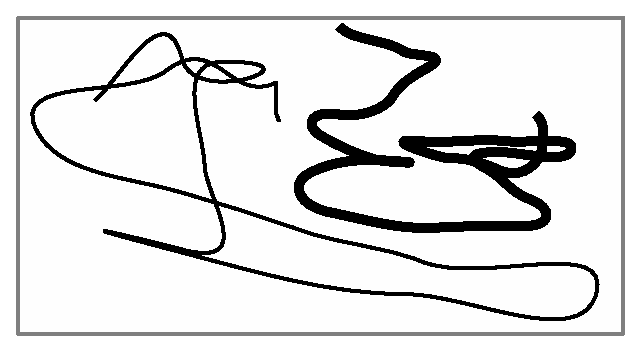
\includegraphics[height=4cm]{fig1}
\caption{Sample EPS figure }
\label{fig1}
\end{center}
\end{figure}

Below is another figure using LaTeX commands.


\begin{figure}[ht]
\begin{center}
\setlength{\unitlength}{1pt}
\footnotesize
\begin{picture}(160,80)
        \put(0,0){\framebox(160,80)[]{}}
        \put(10,35){\framebox(80,40){}}
        \put(100,20){\framebox(40,20){}}
        \put(70,10){\framebox(20,10){}}
        \put(20,5){\framebox(10,5){}}
\end{picture}
\caption{Sample Figure Caption}
\end{center}
\end{figure}

\subsubsection{Tables}

All tables must be centered, neat, clean and legible. Do not use pencil
or hand-drawn tables. Table number and title always appear before the
table.

One line space before the table title, one line space after the table
title and one line space after the table. The table title must be
initial caps and each table numbered consecutively.

\begin{table}[ht]
\begin{center}
\caption{Sample Table}

\bigskip

\begin{tabular}{|l|l|r|}
\hline
A & B & 1\\ \hline
C & D & 2\\
E & F & 3\\ \hline
\end{tabular}
\end{center}
\end{table}


\subsubsection{Handling References}

Use a first level heading for the references. References follow the
acknowledgements.


\subsubsection{Acknowledgements}

Use a third level heading for the acknowledgements. All acknowledgements
go at the end of the paper.




%\bibliographystyle{alpha} 
%\bibliography{samplebib}
%inline the .bbl file directly for mailing to authors.

\begin{thebibliography}{Com79}

\bibitem[Com79]{Comer-btree}
D.~Comer.
\newblock The ubiquitous b-tree.
\newblock {\em Computing Surveys}, 11(2):121--137, June 1979.

\bibitem[Knu73]{Knuth-vol3}
D.~E. Knuth.
\newblock {\em The Art of Computer Programming -- Volume 3 / Sorting and
  Searching}.
\newblock Addison-Wesley, 1973.

\end{thebibliography}

\end{document}
